\documentclass[aspectratio=169]{beamer}

\usetheme{Boadilla}
\usefonttheme{professionalfonts}
\setbeamertemplate{navigation symbols}{}
\setbeamertemplate{itemize items}[circle]
\setbeamertemplate{enumerate items}[default]
\setbeamertemplate{headline}{}

\usepackage[utf8]{inputenc}
\usepackage[T1]{fontenc}
\usepackage{lmodern}
\usepackage{amsmath}
\usepackage{booktabs}
\usepackage{tabularx}
\usepackage{array}
\usepackage{hyperref}
\usepackage[strings]{underscore}
\usepackage{listings}
\usepackage{tikz}
\usetikzlibrary{arrows.meta,positioning,fit,calc,shapes.geometric}
\usepackage{xcolor}

\definecolor{courseblue}{HTML}{12355B}
\definecolor{coursegold}{HTML}{C98A2E}
\definecolor{courseice}{HTML}{EEF3F8}
\definecolor{coursegreen}{HTML}{2F6B4F}
\definecolor{coursegray}{HTML}{4B5563}
\definecolor{codebg}{HTML}{F7F9FC}
\definecolor{codecomment}{HTML}{5E6C84}
\definecolor{codestring}{HTML}{0B6E4F}

\setbeamercolor{palette primary}{bg=courseblue,fg=white}
\setbeamercolor{palette secondary}{bg=coursegold,fg=white}
\setbeamercolor{palette tertiary}{bg=courseblue,fg=white}
\setbeamercolor{palette quaternary}{bg=coursegold,fg=white}
\setbeamercolor{structure}{fg=courseblue}
\setbeamercolor{frametitle}{bg=courseice,fg=courseblue}
\setbeamercolor{title}{fg=courseblue}
\setbeamercolor{block title}{bg=courseblue,fg=white}
\setbeamercolor{block body}{bg=courseice,fg=black}
\setbeamercolor{normal text}{fg=black,bg=white}
\setbeamercolor{alerted text}{fg=coursegold}

\setbeamerfont{footline}{size=\scriptsize}

\setbeamertemplate{footline}{
  \leavevmode
  \hbox{
    \begin{beamercolorbox}[wd=.33\paperwidth,ht=2.8ex,dp=1.2ex,leftskip=0.8em]{palette primary}%
      University of Trieste
    \end{beamercolorbox}%
    \begin{beamercolorbox}[wd=.49\paperwidth,ht=2.8ex,dp=1.2ex,center]{palette tertiary}%
      \coursename{} \textbar{} \coursecode
    \end{beamercolorbox}%
    \begin{beamercolorbox}[wd=.18\paperwidth,ht=2.8ex,dp=1.2ex,rightskip=0.8em plus1fil]{palette secondary}%
      \insertframenumber{} / \inserttotalframenumber
    \end{beamercolorbox}%
  }
}

\hypersetup{
  colorlinks=true,
  linkcolor=courseblue,
  urlcolor=coursegreen
}

\lstdefinestyle{coursepython}{
  language=Python,
  basicstyle=\ttfamily\footnotesize,
  keywordstyle=\color{courseblue}\bfseries,
  commentstyle=\color{codecomment}\itshape,
  stringstyle=\color{codestring},
  showstringspaces=false,
  columns=fullflexible,
  keepspaces=true,
  frame=single,
  framerule=0.6pt,
  rulecolor=\color{courseblue},
  backgroundcolor=\color{codebg},
  xleftmargin=0.4em,
  xrightmargin=0.4em,
  aboveskip=0.4em,
  belowskip=0.2em
}

\newcommand{\coursename}{Data-driven Systems Engineering}
\newcommand{\coursecode}{440MI / 305SM}
\newcommand{\coursefooter}{}

\newcommand{\learninggoals}[1]{
  \begin{block}{Learning goals}
  #1
  \end{block}
}

\newcommand{\repoactivity}[1]{
  \begin{block}{Repo activity}
  #1
  \end{block}
}

\newcommand{\readinglist}[1]{
  \begin{block}{Papers and materials}
  {\footnotesize #1}
  \end{block}
}

\newcommand{\coursecontextframe}[5]{
  \begin{frame}{Course Map and Running Cases}
  \centering
  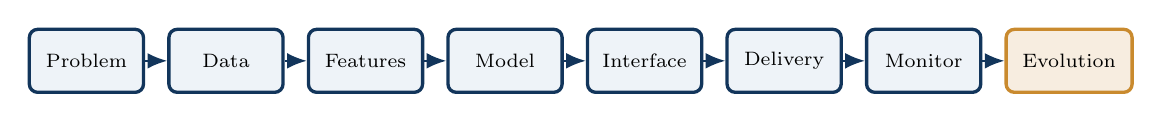
\begin{tikzpicture}[node distance=0.28cm]
  \node[flowbox, minimum width=1.45cm, minimum height=0.8cm] (problem) {\scriptsize Problem};
  \node[flowbox, minimum width=1.45cm, minimum height=0.8cm, right=of problem] (data) {\scriptsize Data};
  \node[flowbox, minimum width=1.45cm, minimum height=0.8cm, right=of data] (features) {\scriptsize Features};
  \node[flowbox, minimum width=1.45cm, minimum height=0.8cm, right=of features] (model) {\scriptsize Model};
  \node[flowbox, minimum width=1.45cm, minimum height=0.8cm, right=of model] (interface) {\scriptsize Interface};
  \node[flowbox, minimum width=1.45cm, minimum height=0.8cm, right=of interface] (delivery) {\scriptsize Delivery};
  \node[flowbox, minimum width=1.45cm, minimum height=0.8cm, right=of delivery] (monitor) {\scriptsize Monitor};
  \node[accentbox, minimum width=1.6cm, minimum height=0.8cm, right=of monitor] (evolution) {\scriptsize Evolution};
  \foreach \a/\b in {problem/data,data/features,features/model,model/interface,interface/delivery,delivery/monitor,monitor/evolution} {
    \draw[arrow] (\a) -- (\b);
  }
  \end{tikzpicture}

  \vspace{0.5em}
  \begin{block}{Today in the course}
  \textbf{Focus:} #1

  \textbf{Bridge:} #2
  \end{block}

  \begin{columns}[T]
  \column{0.48\textwidth}
  \begin{block}{Fraud case}
  {\footnotesize #3}
  \end{block}
  \column{0.48\textwidth}
  \begin{block}{Pasteurization case}
  {\footnotesize #4}
  \end{block}
  \end{columns}

  \vspace{0.3em}
  {\footnotesize \textbf{Course thread:} #5}
  \coursefooter
  \end{frame}
}

\newcommand{\classclosingframe}[4]{
  \begin{frame}{From This Class to the Next}
  \begin{block}{What stays with us}
  #1
  \end{block}

  \begin{columns}[T]
  \column{0.48\textwidth}
  \begin{block}{Project use}
  {\footnotesize #2}
  \end{block}
  \column{0.48\textwidth}
  \begin{block}{Next connection}
  {\footnotesize #3}
  \end{block}
  \end{columns}

  \vspace{0.3em}
  {\footnotesize \textbf{Course thread:} #4}
  \coursefooter
  \end{frame}
}

\tikzset{
  flowbox/.style={
    rounded corners=3pt,
    draw=courseblue,
    fill=courseice,
    very thick,
    minimum width=2.2cm,
    minimum height=0.9cm,
    align=center,
    font=\small
  },
  accentbox/.style={
    rounded corners=3pt,
    draw=coursegold,
    fill=coursegold!15,
    very thick,
    minimum width=2.2cm,
    minimum height=0.9cm,
    align=center,
    font=\small
  },
  arrow/.style={
    -{Latex[length=2.5mm,width=2mm]},
    thick,
    draw=courseblue
  }
}


% Slides read better without automatic hyphenation.
\hyphenpenalty=10000
\exhyphenpenalty=10000

\usetikzlibrary{backgrounds}
\usepackage{colortbl}
\definecolor{coursered}{HTML}{A23B2A}
\newcommand{\goldink}{\color{coursegold!65!black}}

\tikzset{
  tile/.style={rounded corners=4pt, fill=courseice, draw=none, align=center, font=\footnotesize, inner sep=5pt},
  tileblue/.style={tile, fill=white, draw=courseblue!55, thick},
  tilegold/.style={tile, fill=coursegold!14, draw=coursegold, thick},
  tilegreen/.style={tile, fill=coursegreen!10, draw=coursegreen!70, thick},
  tilered/.style={tile, fill=coursered!8, draw=coursered!70, thick},
  tag/.style={rounded corners=2pt, fill=coursegold, text=white, font=\bfseries\tiny, inner sep=2.5pt},
  chip/.style={rounded corners=3pt, fill=courseblue, text=white, font=\footnotesize\bfseries, align=center, inner sep=4pt},
  note/.style={font=\scriptsize, text=coursegray, align=left},
  arrowgold/.style={-{Latex[length=2.5mm,width=2mm]}, thick, draw=coursegold},
  arrowred/.style={-{Latex[length=2.5mm,width=2mm]}, thick, draw=coursered},
  arrowgray/.style={-{Latex[length=2mm,width=1.6mm]}, thick, draw=coursegray!70},
}

% Footer: a strip with the concepts that appear for the first time on the slide, above the
% usual bar. The bar total counts only the main lecture; the backup slide is numbered separately.
\makeatletter
\def\conceptstext{}
\def\currentsectionname{}
\setbeamercolor{conceptbar}{bg=coursegold!12,fg=black}
\newcommand{\cterm}[2]{{\bfseries\color{courseblue}#1:}\ #2\hspace{0.8em}}
\newcommand{\newtag}{\colorbox{coursegold}{\color{white}\bfseries\tiny\ NEW\ }\hspace{0.6em}}
\setbeamertemplate{footline}{
  \leavevmode
  \vbox{%
    \ifx\conceptstext\empty\else
      \hbox{\color{coursegold}\rule{\paperwidth}{0.8pt}}%
      \hbox{\begin{beamercolorbox}[wd=\paperwidth,leftskip=0.5cm,rightskip=0.5cm,sep=3pt]{conceptbar}\scriptsize\newtag\conceptstext\end{beamercolorbox}}%
    \fi
    \hbox{%
      \begin{beamercolorbox}[wd=.33\paperwidth,ht=2.8ex,dp=1.2ex,leftskip=0.8em]{palette primary}%
        \ifbeamer@inappendix Backup\else\ifnum\value{section}>0 \arabic{section}\ \textbar\ \currentsectionname\else University of Trieste\fi\fi
      \end{beamercolorbox}%
      \begin{beamercolorbox}[wd=.49\paperwidth,ht=2.8ex,dp=1.2ex,center]{palette tertiary}%
        \coursename{} \textbar{} \coursecode
      \end{beamercolorbox}%
      \begin{beamercolorbox}[wd=.18\paperwidth,ht=2.8ex,dp=1.2ex,right,rightskip=0.8em]{palette secondary}%
        \ifbeamer@inappendix Backup \insertframenumberinappendix\else\insertframenumber{} / \insertmainframenumber\fi
      \end{beamercolorbox}%
    }}}
\makeatother
\newenvironment{cframe}[2]{\gdef\conceptstext{#2}\begin{frame}{#1}}{\end{frame}\gdef\conceptstext{}}


% Section dividers: progress strip, recap of the previous part, and the roadmap of the next one.
\newcommand{\sectiondivider}[4]{% number title previously items
  \section{#2}\gdef\currentsectionname{#2}
  \begin{frame}
  \centering
  \begin{tikzpicture}
  \foreach \i/\lab in {1/SE and ML,2/Requirements,3/Process,4/Design,5/Quality,6/Evolution} {
    \ifnum\i<#1 \def\chipfill{courseblue!22}\def\chiptext{courseblue}\else
    \ifnum\i=#1 \def\chipfill{courseblue}\def\chiptext{white}\else
    \def\chipfill{courseice}\def\chiptext{coursegray}\fi\fi
    \node[rounded corners=3pt, minimum width=2.15cm, minimum height=0.6cm, font=\scriptsize\bfseries, fill=\chipfill, text=\chiptext] at ({1.075+(\i-1)*2.25},0) {\i\ \lab};
  }
  \node[circle, fill=courseblue, text=white, font=\Huge\bfseries, minimum size=1.7cm, inner sep=0] at (1.0,-1.7) {#1};
  \node[anchor=west, font=\huge\bfseries, text=courseblue, text width=11cm, align=left] at (2.2,-1.7) {#2};
  \ifx\relax#3\relax\else
    \node[anchor=north west, font=\small\itshape, text=coursegray, text width=13.2cm, align=left] at (0.1,-2.75) {Previously: #3};
  \fi
  \node[anchor=north west, font=\footnotesize\bfseries, text=coursegold!65!black] at (0.1,-3.45) {IN THIS PART};
  \node[anchor=north west, font=\small, text width=13.2cm, align=left] at (0.1,-3.85) {#4};
  \end{tikzpicture}
  \end{frame}
}
\newcommand{\principletag}[1]{%
  \begin{tikzpicture}[remember picture, overlay]
    \node[tag, anchor=north east] at ([xshift=-0.35cm,yshift=-0.3cm]current page.north east) {PRINCIPLE #1 OF 4};
  \end{tikzpicture}%
}

\title{Class 20: Introduction to Software Engineering for Data Products}
\subtitle{Session 20 of 36 -- Opening the Software Engineering and MLOps Block}
\author{\coursename}
\date{}

\begin{document}

\frame{\titlepage \coursefooter}

% ------------------------------------------------------------------ agenda
\newcommand{\agendacard}[5]{% x y number title description
  \node[tile, anchor=north west, minimum width=4.3cm, minimum height=1.85cm] (card#3) at (#1,#2) {};
  \node[circle, fill=courseblue, text=white, font=\bfseries, minimum size=0.78cm, inner sep=0] at ([shift={(0.62,-0.7)}]card#3.north west) {#3};
  \node[anchor=north west, text width=3.0cm, align=left, font=\footnotesize] at ([shift={(1.08,-0.2)}]card#3.north west) {\textbf{\color{courseblue}#4}\\[2pt]{\scriptsize\color{coursegray}#5}};
}

\begin{frame}{Agenda}
\centering
\begin{tikzpicture}
\agendacard{0}{0}{1}{Software engineering and ML}{From programming to engineering}
\agendacard{4.55}{0}{2}{Requirements and quality}{Attributes, functional and non-functional}
\agendacard{9.1}{0}{3}{Process and system types}{Four activities, two running cases}
\agendacard{0}{-2.1}{4}{Design}{Modularity, coupling, interfaces}
\agendacard{4.55}{-2.1}{5}{Quality assurance}{Testing code, data, and models}
\agendacard{9.1}{-2.1}{6}{Evolution and MLOps}{Maintenance and DevOps}
\end{tikzpicture}
\coursefooter
\end{frame}

% ------------------------------------------------------------------ what is software engineering
\newcommand{\sedim}[6]{% x style title subtitle text index
  \node[#2, anchor=north west, minimum width=3.2cm, minimum height=2.9cm] (sd#6) at (#1,2.3) {};
  \node[anchor=north west, text width=2.85cm, align=left, inner sep=0pt, font=\scriptsize] at ([shift={(0.17,-0.17)}]sd#6.north west) {{\small\bfseries\color{courseblue}#3}\\[1pt]{\itshape\color{coursegray}#4}\\[5pt]#5};
}
\sectiondivider{1}{Software engineering and ML}{}{$\bullet$\ From programming to software engineering\\[3pt]$\bullet$\ A model is one box in a system}

\begin{cframe}{From programming to software engineering}{\cterm{Trade-off}{gaining one quality by giving up another, e.g.\ speed for cost.}\cterm{Dependable}{behaving correctly when it matters, without causing harm.}}
\centering
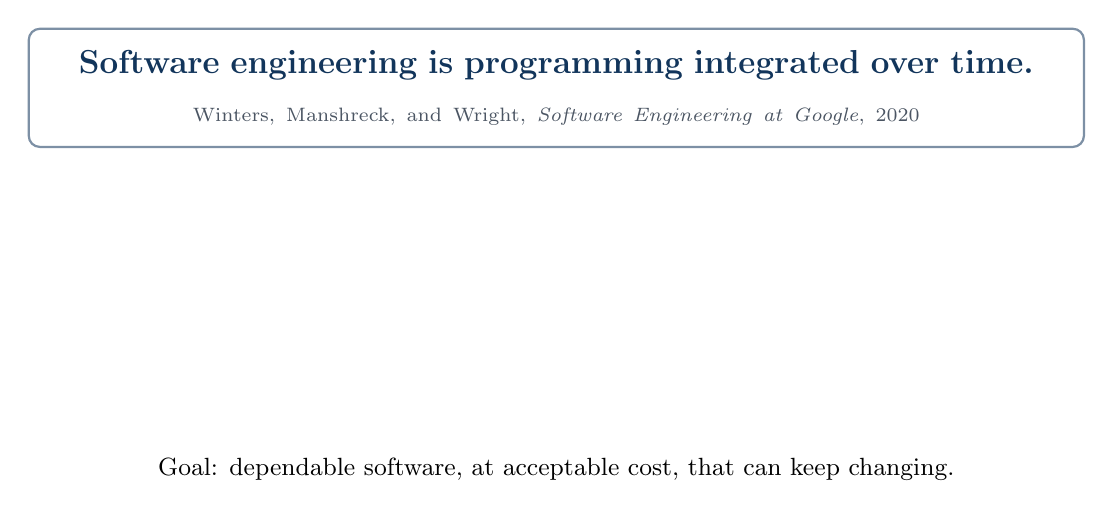
\begin{tikzpicture}
\node[tileblue, minimum width=13.4cm, text width=12.8cm, inner sep=8pt, font=\large] at (6.7,3.6) {\textbf{\color{courseblue}Software engineering is programming integrated over time.}\\[3pt]{\scriptsize\color{coursegray} Winters, Manshreck, and Wright, \emph{Software Engineering at Google}, 2020}};
\sedim{0}{tile}{Time}{how long it lives}{Maintained, upgraded, and eventually replaced long after it was written.}{1}
\sedim{3.4}{tile}{Scale}{size and reach}{More users, data, and dependencies, and more ways to fail.}{2}
\sedim{6.8}{tile}{Trade-offs}{hard choices}{Cost, risk, and deadlines force choices that someone must later explain.}{3}
\sedim{10.2}{tilegold}{Data}{added by ML}{The system changes without a code change: data shifts and models are retrained.}{4}
\node[font=\small] at (6.7,-1.25) {Goal: dependable software, at acceptable cost, that can keep changing.};
\end{tikzpicture}
\coursefooter
\end{cframe}

% ------------------------------------------------------------------ model vs system
\begin{cframe}{A model is one box in a system}{\cterm{Serving}{making a trained model answer requests.}\cterm{Monitoring}{watching a running system and its data.}}
\centering
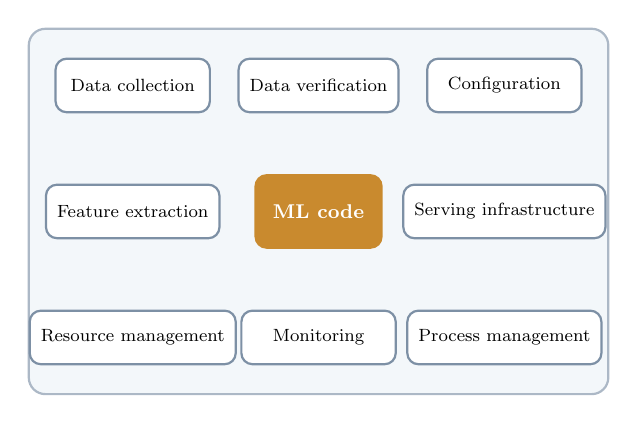
\begin{tikzpicture}[scale=0.8, transform shape]
\draw[rounded corners=6pt, draw=courseblue!35, fill=courseice!70, thick] (-0.3,-0.3) rectangle (8.9,5.5);
\tikzset{sys/.style={tileblue, minimum width=2.45cm, minimum height=0.85cm},
         rep/.style={tile, fill=white, draw=coursegold, very thick, minimum width=2.45cm, minimum height=0.85cm}}
\node[sys] at (1.35,4.6) {Data collection};
\node[sys] at (4.3,4.6) {Data verification};
\node[sys] at (7.25,4.6) {Configuration};
\node[sys] at (1.35,2.6) {Feature extraction};
\node[tilegold, minimum width=2.0cm, minimum height=1.15cm, font=\bfseries\small, fill=coursegold, text=white] at (4.3,2.6) {ML code};
\node[sys] at (7.25,2.6) {Serving infrastructure};
\node[sys] at (1.35,0.6) {Resource management};
\node[sys] at (4.3,0.6) {Monitoring};
\node[sys] at (7.25,0.6) {Process management};
\end{tikzpicture}

{\small The model is the small part; the rest decides whether it works in practice.}

{\tiny\color{coursegray} Redrawn after Sculley et al., NeurIPS 2015; schematic, not to scale.}
\coursefooter
\end{cframe}

% ------------------------------------------------------------------ attributes
\newcommand{\attrrow}[5]{% y label why kpis returns
  \node[chip, minimum width=2.45cm, minimum height=0.7cm, font=\scriptsize\bfseries] at (1.225,#1) {#2};
  \node[anchor=west, text width=3.25cm, font=\scriptsize, align=left] at (2.65,#1) {#3};
  \node[anchor=west, text width=3.9cm, font=\scriptsize\bfseries, align=left, text=courseblue] at (6.2,#1) {#4};
  \node[anchor=west, text width=3.3cm, font=\scriptsize, align=left] at (10.4,#1) {#5};
  \draw[courseice!70!courseblue, line width=0.5pt] (0,#1-0.45) -- (13.7,#1-0.45);
}

\sectiondivider{2}{Requirements and quality}{the model is the small part; the system around it decides whether it works.}{$\bullet$\ Quality attributes and their KPIs\\[3pt]$\bullet$\ Requirements come before implementation\\[3pt]$\bullet$\ Functional and non-functional requirements}

\begin{cframe}{Quality attributes of ML-enabled software}{\cterm{KPI}{a measurable indicator of a goal.}\cterm{Latency (p95)}{time from request to response; p95 means 95\% of requests are faster.}\cterm{Availability}{share of time the system works.}\cterm{Traceability}{following a decision back to its sources.}\cterm{Rollback}{going back to the previous version.}}
\centering
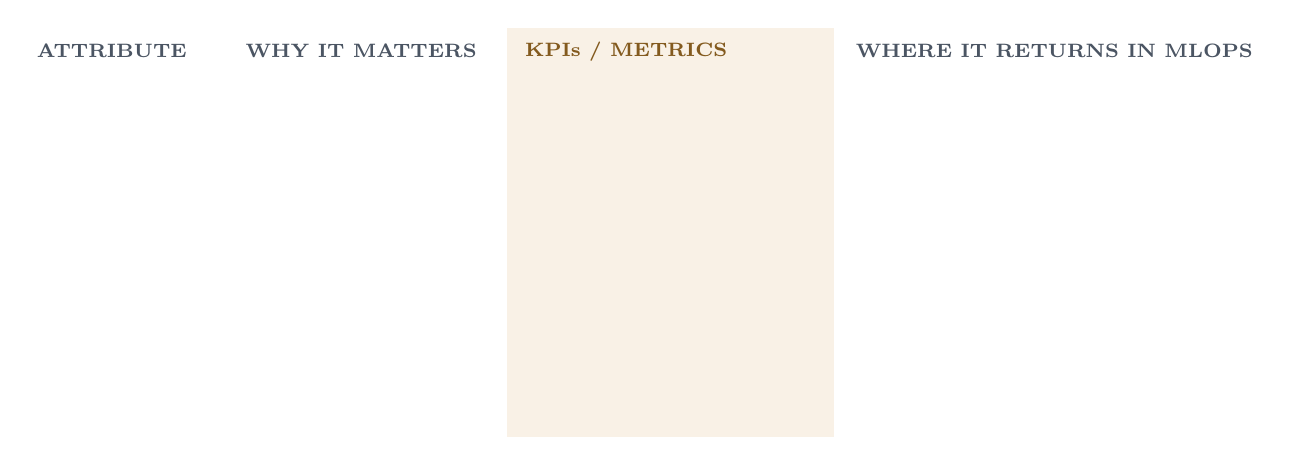
\begin{tikzpicture}
\fill[coursegold!12] (6.1,-0.9) rectangle (10.25,4.3);
\node[anchor=west, font=\scriptsize\bfseries, text=coursegray] at (0,4.0) {ATTRIBUTE};
\node[anchor=west, font=\scriptsize\bfseries, text=coursegray] at (2.65,4.0) {WHY IT MATTERS};
\node[anchor=west, font=\scriptsize\bfseries, text=coursegold!65!black] at (6.2,4.0) {KPIs / METRICS};
\node[anchor=west, font=\scriptsize\bfseries, text=coursegray] at (10.4,4.0) {WHERE IT RETURNS IN MLOPS};
\attrrow{3.2}{Maintainability}{Models, features, and infrastructure all change.}{Modules touched per change; test coverage}{Modular pipelines and automated tests.}
\attrrow{2.3}{Dependability}{Wrong predictions can cause harm.}{Availability; error rate; recall on fraud}{Monitoring, alerts, and rollback.}
\attrrow{1.4}{Efficiency}{Latency and compute cost decide feasibility.}{p95 latency; requests per second; cost per 1,000 predictions}{Serving, batching, and scaling.}
\attrrow{0.5}{Usability}{Operators must understand outputs.}{Task success rate; time to decision}{Decision-support interfaces.}
\attrrow{-0.4}{Traceability}{Decisions must be auditable afterward.}{Share of predictions logged with model version}{Versioning and audit logs.}
\end{tikzpicture}
\coursefooter
\end{cframe}

% ------------------------------------------------------------------ requirements: iceberg
\begin{cframe}{Requirements come before implementation}{\cterm{Functional requirement}{what the system does.}\cterm{Non-functional requirement}{how well it does it.}\cterm{Service}{a program that keeps running and answers other programs through an agreed interface.}\cterm{API}{the set of operations a service offers.}}
\begin{columns}[T]
\column{0.50\textwidth}
\centering
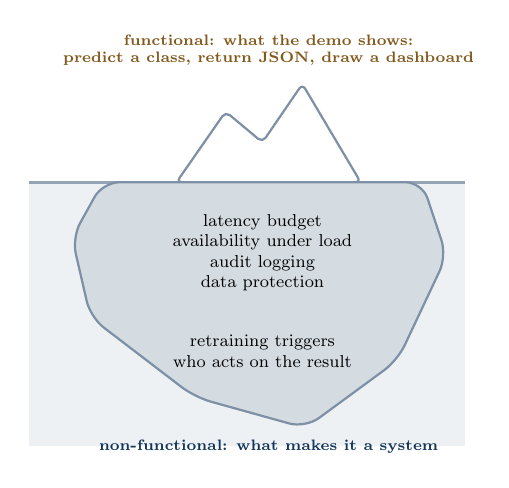
\begin{tikzpicture}[scale=0.78, transform shape]
\fill[courseblue!7] (-0.5,-4.3) rectangle (6.6,0);
\draw[courseblue!45, line width=1pt] (-0.5,0) -- (6.6,0);
\fill[white, draw=courseblue!55, thick, rounded corners=2pt] (1.9,0) -- (2.7,1.15) -- (3.3,0.65) -- (3.95,1.6) -- (4.9,0) -- cycle;
\fill[courseblue!18, draw=courseblue!55, thick, rounded corners=6pt]
  (0.7,0) -- (5.9,0) -- (6.3,-1.2) -- (5.5,-2.9) -- (4.0,-4.0) -- (2.2,-3.5) -- (0.5,-2.2) -- (0.2,-0.9) -- cycle;
\node[font=\scriptsize\bfseries, text=coursegold!65!black, align=center] at (3.4,2.15) {functional: what the demo shows:\\predict a class, return JSON, draw a dashboard};
\node[font=\footnotesize, text=black, text width=4.6cm, align=center] at (3.3,-1.15) {latency budget\\availability under load\\audit logging\\data protection};
\node[font=\footnotesize, text=black, text width=4.4cm, align=center] at (3.3,-2.75) {retraining triggers\\who acts on the result};
\node[font=\scriptsize\bfseries, text=courseblue] at (3.4,-4.3) {non-functional: what makes it a system};
\end{tikzpicture}
\column{0.47\textwidth}
\begin{itemize}
\small
\item Software engineering starts by clarifying what the system must do and how well.
\item A strong model does not rescue unclear goals or vague success criteria.
\item Many ML failures are non-functional: the model exists, but the service is slow, brittle, or opaque.
\item In data products, requirements cover software behavior and data behavior.
\end{itemize}
\end{columns}
\coursefooter
\end{cframe}

\newcommand{\Ftag}{\colorbox{courseblue}{\color{white}\bfseries\scriptsize\ \ F\ \ }}
\newcommand{\NFtag}{\colorbox{coursegold}{\color{white}\bfseries\scriptsize\ NF\ }}
\begin{cframe}{Functional and non-functional requirements}{\cterm{Acceptance criterion}{a measurable condition that tells us a requirement is met.}\cterm{Load test}{sending many requests at once to see how the system behaves.}\cterm{Contract test}{checks that a service still honors its API.}}
\centering
{\small \Ftag\ \textbf{Functional:} what the system does \qquad\quad \NFtag\ \textbf{Non-functional:} how well it does it}

\vspace{0.6em}
\renewcommand{\arraystretch}{1.25}
\setlength{\tabcolsep}{5pt}
{\footnotesize
\begin{tabularx}{\textwidth}{>{\centering\arraybackslash}p{1.0cm} >{\raggedright\arraybackslash}X >{\raggedright\arraybackslash}p{2.5cm} >{\raggedright\arraybackslash}p{3.4cm}}
\rowcolor{courseblue}
\color{white}\textbf{Type} & \color{white}\textbf{Requirement (example)} & \color{white}\textbf{Quality attribute} & \color{white}\textbf{How we check it} \\
\rowcolor{courseice}
\Ftag & Return a fraud probability and decision. & \textcolor{coursegray}{--} & Input/output tests \\
\rowcolor{courseice}
\Ftag & Show live sensor readings on a dashboard. & \textcolor{coursegray}{--} & Acceptance check \\
\rowcolor{coursegold!12}
\NFtag & Swap the model without changing the API. & Maintainability & Contract tests on swap \\
\rowcolor{coursegold!5}
\NFtag & Reject invalid input with HTTP 400. & Dependability & Invalid-input tests \\
\rowcolor{coursegold!12}
\NFtag & 95\% of requests answered within 800 ms. & Efficiency & Load test; p95 latency \\
\rowcolor{coursegold!5}
\NFtag & Show the probability and threshold. & Usability & Review with operators \\
\rowcolor{coursegold!12}
\NFtag & Log each prediction and model version. & Traceability & Inspect the log \\
\end{tabularx}}

\vspace{0.5em}
{\small Non-functional requirements are quality attributes made measurable.}
\end{cframe}

% ------------------------------------------------------------------ process
\sectiondivider{3}{Process and system types}{quality attributes become measurable requirements.}{$\bullet$\ Four activities, one loop\\[3pt]$\bullet$\ Kinds of software systems\\[3pt]$\bullet$\ A data collection system: the pasteurization stream}

\begin{cframe}{Four activities, one loop}{\cterm{Validation}{checking that we built the right thing (verification: that we built it right).}\cterm{Label}{the true outcome of a case, e.g.\ fraud or not.}\cterm{Data distribution}{how values are spread; it can shift over time.}}
\centering
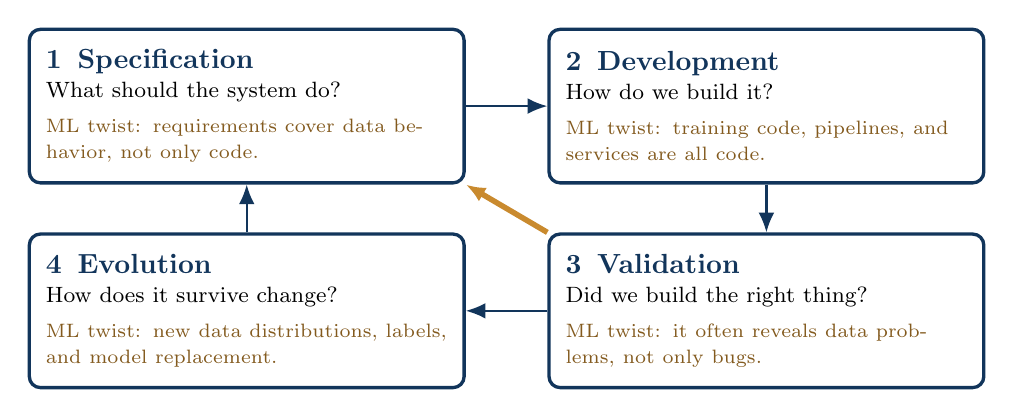
\begin{tikzpicture}
\tikzset{act/.style={tile, fill=white, draw=courseblue, very thick, text width=5.1cm, minimum height=1.95cm, align=left, inner sep=6pt}}
\node[act] (spec) at (-3.3,1.3) {\textbf{\color{courseblue}\normalsize 1\ \ Specification}\\[1pt]What should the system do?\\[3pt]{\scriptsize\goldink ML twist: requirements cover data behavior, not only code.}};
\node[act] (dev) at (3.3,1.3) {\textbf{\color{courseblue}\normalsize 2\ \ Development}\\[1pt]How do we build it?\\[3pt]{\scriptsize\goldink ML twist: training code, pipelines, and services are all code.}};
\node[act] (val) at (3.3,-1.3) {\textbf{\color{courseblue}\normalsize 3\ \ Validation}\\[1pt]Did we build the right thing?\\[3pt]{\scriptsize\goldink ML twist: it often reveals data problems, not only bugs.}};
\node[act] (evo) at (-3.3,-1.3) {\textbf{\color{courseblue}\normalsize 4\ \ Evolution}\\[1pt]How does it survive change?\\[3pt]{\scriptsize\goldink ML twist: new data distributions, labels, and model replacement.}};
\draw[arrow] (spec.east) -- (dev.west);
\draw[arrow] (dev.south) -- (val.north);
\draw[arrow] (val.west) -- (evo.east);
\draw[arrow] (evo.north) -- (spec.south);
\draw[arrowgold, line width=2pt] (val.north west) -- (spec.south east);
\end{tikzpicture}

{\scriptsize\color{coursegray} The gold arrow: validation often sends us back to the specification, because data problems show up as requirement problems.}
\coursefooter
\end{cframe}

% ------------------------------------------------------------------ kinds of systems
\newcommand{\casetag}[1]{\\[4pt]\colorbox{coursegold}{\color{white}\bfseries\tiny\ #1\ }}
\newcommand{\systile}[7]{% name x y style title example tag
  \node[#4, minimum width=4.35cm, minimum height=2.1cm, text width=3.95cm] (#1) at (#2,#3) {\textbf{#5}\\[2pt]{\scriptsize\color{coursegray}#6}#7};
}
\begin{cframe}{Kinds of software systems}{\cterm{Transaction-based}{a request in, an answer out.}\cterm{Batch}{many items processed together, on a schedule.}\cterm{Embedded}{software inside a device.}\cterm{System of systems}{independent systems that cooperate.}\cterm{CRM}{customer-management software.}}
\centering
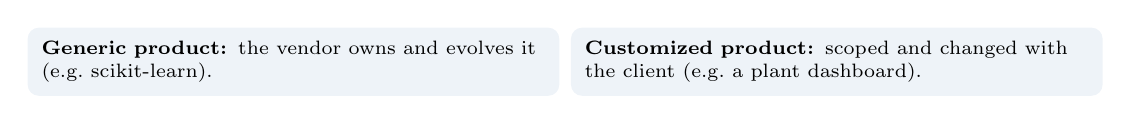
\begin{tikzpicture}
\systile{s1}{0}{0}{tileblue}{Stand-alone application}{A Streamlit dashboard running on one laptop}{}
\systile{s2}{4.65}{0}{tilegold}{Transaction-based system}{Fraud scoring API: request in, answer out}{\casetag{FRAUD CASE}}
\systile{s3}{9.3}{0}{tileblue}{Embedded control system}{The pasteurizer's own controller (outside our scope)}{}
\systile{s4}{0}{-2.3}{tileblue}{Batch processing system}{Scheduled retraining (Class 27)}{}
\systile{s5}{4.65}{-2.3}{tilegold}{Data collection system}{Sensor stream feeding an online predictor}{\casetag{PASTEURIZATION CASE}}
\systile{s6}{9.3}{-2.3}{tileblue}{System of systems}{Model service + feature pipeline + CRM + alert routing}{}
\node[tile, minimum width=6.7cm, text width=6.4cm, align=left, font=\scriptsize] at (2.2,-4.4) {\textbf{Generic product:} the vendor owns and evolves it (e.g.\ scikit-learn).};
\node[tile, minimum width=6.7cm, text width=6.4cm, align=left, font=\scriptsize] at (9.1,-4.4) {\textbf{Customized product:} scoped and changed with the client (e.g.\ a plant dashboard).};
\end{tikzpicture}
\coursefooter
\end{cframe}

% ------------------------------------------------------------------ pasteurization stream
\begin{cframe}{A data collection system: the pasteurization stream}{\cterm{Stream}{data pushed continuously, one event at a time.}\cterm{Event}{one message, here a sensor reading with its timestamp.}\cterm{Server-Sent Events (SSE)}{a web protocol for a server to push events to a client.}\cterm{Timeliness, continuity}{readings arrive on time and without gaps.}}
\centering
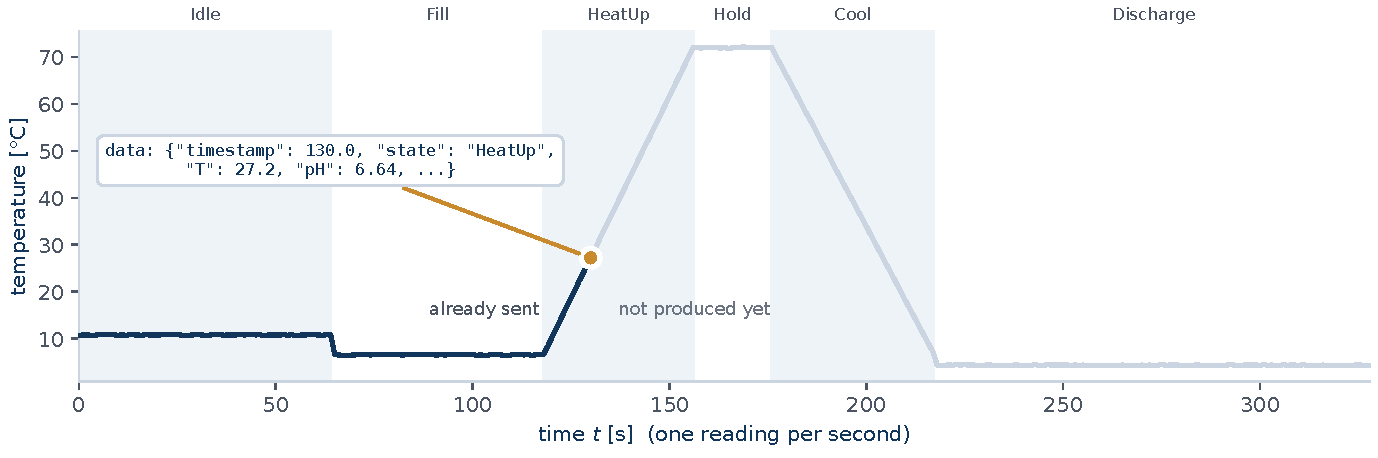
\includegraphics[width=0.93\textwidth,height=0.55\textheight,keepaspectratio]{images/class20_sse_stream.pdf}
\begin{itemize}\small
\item The server pushes one event per reading: a continuous flow, not a request and a reply.
\item Its quality attributes differ from the fraud API: timeliness and continuity matter more than the latency of one call.
\end{itemize}
\coursefooter
\end{cframe}

% ------------------------------------------------------------------ design principles
\newcommand{\ptile}[6]{% x y style title definition ML-example
  \node[#3, anchor=north west, minimum width=6.55cm, minimum height=2.4cm, text width=6.15cm, align=left] at (#1,#2) {{\normalsize\bfseries\color{courseblue}#4}\\[3pt]#5\\[4pt]{\scriptsize\goldink\textbf{In ML systems:} #6}};
}
% ------------------------------------------------------------------ design principle 1: modularity
\sectiondivider{4}{Design}{we know what to build; now, how to structure it.}{$\bullet$\ Four parallel principles: modularity, high cohesion, low coupling, interface as contract\\[3pt]$\bullet$\ Change scenarios: who has to change?\\[3pt]$\bullet$\ Example: a prediction service as a pipeline of responsibilities}

\begin{cframe}{Modularity: decompose by what is likely to change}{\cterm{Module}{a part with one clear responsibility and a boundary.}\cterm{Interface}{how other parts use a module.}\cterm{Information hiding}{a module keeps one design decision private, so changing it does not ripple out.}}
\principletag{1}
\begin{columns}[T]
\column{0.57\textwidth}
\centering
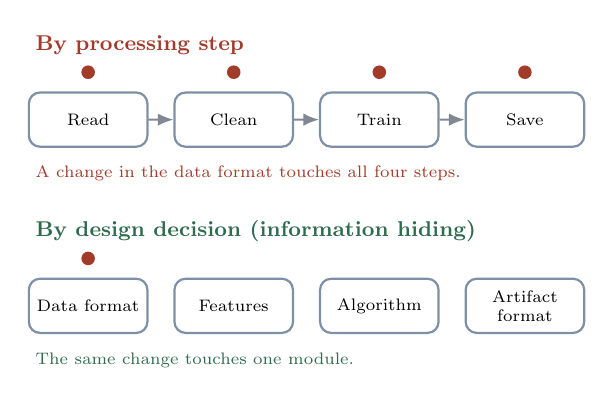
\begin{tikzpicture}[scale=0.86, transform shape]
\tikzset{mm/.style={tileblue, minimum width=1.75cm, minimum height=0.8cm, font=\scriptsize, inner sep=2pt}}
\node[font=\small\bfseries, text=coursered, anchor=west] at (0,4.7) {By processing step};
\foreach \i/\lab in {1/Read,2/Clean,3/Train,4/Save} {
  \node[mm] (a\i) at ({0.9+(\i-1)*2.15},3.6) {\lab};
  \fill[coursered] ({0.9+(\i-1)*2.15},4.3) circle (0.1);
}
\foreach \i/\j in {1/2,2/3,3/4} {\draw[arrowgray] (a\i) -- (a\j);}
\node[font=\scriptsize, text=coursered, anchor=west] at (0,2.8) {A change in the data format touches all four steps.};
\node[font=\small\bfseries, text=coursegreen, anchor=west] at (0,1.95) {By design decision (information hiding)};
\foreach \i/\lab in {1/Data format,2/Features,3/Algorithm,4/Artifact\\format} {
  \node[mm] (b\i) at ({0.9+(\i-1)*2.15},0.85) {\lab};
}
\fill[coursered] (0.9,1.55) circle (0.1);
\node[font=\scriptsize, text=coursegreen, anchor=west] at (0,0.05) {The same change touches one module.};
\end{tikzpicture}
\column{0.40\textwidth}
\small
\begin{itemize}\setlength{\itemsep}{5pt}
\item A \textbf{module} has a responsibility, a public interface, and hidden internals.
\item \textbf{Information hiding} (Parnas, 1972): each module hides one design decision likely to change.
\item \textbf{Benefits:} independent work, testing alone, replacement, reuse.
\item \textbf{Cost:} interfaces take effort; many tiny modules are as bad as one big one.
\end{itemize}
\end{columns}
\coursefooter
\end{cframe}

\begin{cframe}{Modularity in practice: the wine project (Class 19)}{\cterm{Artifact}{a file produced by training and deployed, e.g.\ a model file.}\cterm{Hyperparameter}{a setting chosen before training.}\cterm{Sweep}{a systematic search over hyperparameter values.}\cterm{Model registry}{a catalog of versioned models, with promotion rules.}}
\principletag{1}
\centering
{\small One file per responsibility; each one hides a decision that is likely to change.}

\vspace{0.5em}
\renewcommand{\arraystretch}{1.35}
\setlength{\tabcolsep}{5pt}
{\scriptsize
\begin{tabularx}{\textwidth}{>{\raggedright\arraybackslash}p{2.3cm} >{\raggedright\arraybackslash}X >{\raggedright\arraybackslash}p{3.3cm} >{\raggedright\arraybackslash}p{4.0cm}}
\rowcolor{courseblue}
\color{white}\textbf{Module} & \color{white}\textbf{Responsibility} & \color{white}\textbf{Decision it hides} & \color{white}\textbf{A change that stays inside} \\
\texttt{configs/*.yaml} & The settings of each run & Hyperparameters and search space & Try new values without editing code \\
\rowcolor{courseice}
\texttt{train.py} & Fit a model, save the artifact & Model family, training loop & Swap the model, keep the rest \\
\texttt{sweep.py} & Run a hyperparameter sweep & Search strategy & Switch the search method \\
\rowcolor{courseice}
\texttt{evaluate.py} & Evaluate once on the test set & Metrics, test protocol & Add a metric \\
\texttt{register.py} & Promote an artifact to the registry & Promotion rules & Tighten the release gate \\
\rowcolor{courseice}
\texttt{figures.py} & Draw the report figures & Plot style and layout & Restyle without retraining \\
\end{tabularx}}

\vspace{0.4em}
{\scriptsize\color{coursegray} Source: the \texttt{wine-wandb} project, Class 19 (repository connections).}
\coursefooter
\end{cframe}

% ------------------------------------------------------------------ design principle 2: cohesion
\begin{cframe}{High cohesion: one module, one reason to change}{\cterm{Cohesion}{how closely the parts of a module belong together.}\cterm{Responsibility}{one job a module is in charge of.}}
\principletag{2}
\begin{columns}[T]
\column{0.38\textwidth}
\centering
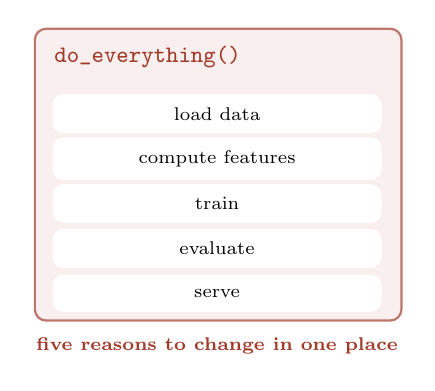
\begin{tikzpicture}[scale=0.95, transform shape]
\node[tilered, anchor=north west, minimum width=4.9cm, minimum height=3.9cm] at (0,0) {};
\node[font=\small\bfseries\ttfamily, anchor=north west, text=coursered] at (0.15,-0.12) {do\_everything()};
\foreach \i/\lab in {1/load data,2/compute features,3/train,4/evaluate,5/serve} {
  \node[tile, fill=white, minimum width=4.4cm, minimum height=0.5cm, font=\scriptsize] at (2.45,{-0.55-\i*0.6}) {\lab};
}
\node[font=\scriptsize\bfseries, text=coursered] at (2.45,-4.25) {five reasons to change in one place};
\end{tikzpicture}
\column{0.60\textwidth}
\renewcommand{\arraystretch}{1.3}
\setlength{\tabcolsep}{4pt}
{\footnotesize
\begin{tabularx}{\linewidth}{>{\raggedright\arraybackslash}p{2.9cm} >{\raggedright\arraybackslash}X}
\rowcolor{courseblue}
\color{white}\textbf{Responsibility} & \color{white}\textbf{Changes when\dots} \\
Load data & the source or the format changes \\
\rowcolor{courseice}
Compute features & a new signal or definition is needed \\
Train & the algorithm or its settings change \\
\rowcolor{courseice}
Evaluate & the metric or the test protocol changes \\
Serve & the API contract changes \\
\end{tabularx}}

\vspace{0.6em}
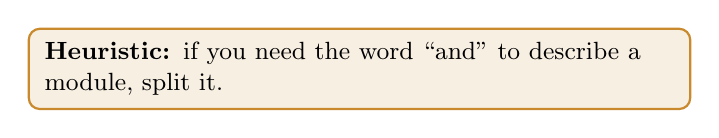
\begin{tikzpicture}
\node[tilegold, anchor=north west, minimum width=8.4cm, text width=8.0cm, align=left, font=\small] at (0,0) {\textbf{Heuristic:} if you need the word ``and'' to describe a module, split it.};
\end{tikzpicture}
\end{columns}
\coursefooter
\end{cframe}

% ------------------------------------------------------------------ design principle 3: coupling
\begin{cframe}{Low coupling: depend on interfaces, not on internals}{\cterm{Coupling}{how much a module depends on another's internals.}\cterm{Schema}{the declared structure of data: names, types, order.}\cterm{Pickle}{Python's format for saving objects; load only trusted files.}\cterm{Session}{one run of a notebook or program.}\cterm{Pin versions}{fix exact library versions.}}
\principletag{3}
\begin{columns}[T]
\column{0.40\textwidth}
\centering
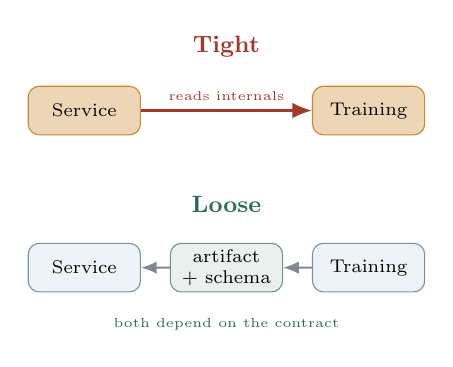
\begin{tikzpicture}[scale=0.95, transform shape]
\tikzset{cn/.style={tile, minimum width=1.5cm, minimum height=0.65cm, font=\scriptsize, inner sep=2pt}}
\node[font=\small\bfseries, text=coursered] at (2.7,3.85) {Tight};
\node[cn, fill=coursegold!35, draw=coursegold] (s1) at (0.8,3.0) {Service};
\node[cn, fill=coursegold!35, draw=coursegold] (t1) at (4.6,3.0) {Training};
\draw[arrowred] (s1) -- node[above, font=\tiny, text=coursered] {reads internals} (t1);
\node[font=\small\bfseries, text=coursegreen] at (2.7,1.75) {Loose};
\node[cn, fill=courseice, draw=courseblue!55] (s2) at (0.8,0.9) {Service};
\node[cn, fill=coursegreen!10, draw=coursegreen!70, minimum width=1.5cm] (c2) at (2.7,0.9) {artifact\\+ schema};
\node[cn, fill=courseice, draw=courseblue!55] (t2) at (4.6,0.9) {Training};
\draw[arrowgray] (t2) -- (c2);
\draw[arrowgray] (c2) -- (s2);
\node[font=\tiny, text=coursegreen] at (2.7,0.15) {both depend on the contract};
\end{tikzpicture}
\column{0.57\textwidth}
{\scriptsize
\renewcommand{\arraystretch}{1.3}
\setlength{\tabcolsep}{4pt}
\begin{tabularx}{\linewidth}{>{\raggedright\arraybackslash}p{1.5cm} >{\raggedright\arraybackslash}X >{\raggedright\arraybackslash}p{2.6cm}}
\rowcolor{courseblue}
\color{white}\textbf{Form} & \color{white}\textbf{Example in ML} & \color{white}\textbf{Loosen by} \\
Content & A dashboard reads private attributes of the model object & Expose a method or a response field \\
\rowcolor{courseice}
Environment & A pickled model loads only with the library version that wrote it & Pin versions; rebuild with the environment \\
Schema & Training and serving each assume the same column order & Define the schema once; validate at the boundary \\
\rowcolor{courseice}
Temporal & Step B only works if step A ran earlier in the session & Explicit inputs and outputs; a pipeline that runs in order \\
\end{tabularx}}
\end{columns}
\coursefooter
\end{cframe}

% ------------------------------------------------------------------ contract in detail
\begin{cframe}{Interface as contract: what to specify}{\cterm{HTTP status}{200 = OK, 400 = invalid request, 500 = server failure.}\cterm{Deterministic}{the same input always gives the same output.}\cterm{Model version}{which artifact produced a response.}}
\principletag{4}
\centering
{\small An interface is a contract: inputs, outputs, and behavior on error are agreed in advance.}\par\vspace{0.4em}
\renewcommand{\arraystretch}{1.1}
\setlength{\tabcolsep}{5pt}
{\scriptsize
\begin{tabularx}{\textwidth}{>{\raggedright\arraybackslash}p{1.9cm} >{\raggedright\arraybackslash}X >{\raggedright\arraybackslash}X}
\rowcolor{courseblue}
\color{white}\textbf{Element} & \color{white}\textbf{Fraud API (request and response)} & \color{white}\textbf{Pasteurization stream (events)} \\
\textbf{Input} & A \texttt{features} list of 30 finite numbers in a fixed order. & None: the client opens the stream and listens. \\
\rowcolor{courseice}
\textbf{Output} & \texttt{fraud\_probability}, \texttt{threshold}, \texttt{is\_fraud}, \texttt{model\_version}, \texttt{request\_id}. & One JSON event per reading: \texttt{timestamp}, \texttt{state}, \texttt{T}, \texttt{pH}, \texttt{Q\_in}, \dots \\
\textbf{Errors} & HTTP 400 with a message; never a silent answer. & The connection closes; the client decides whether to reconnect. \\
\rowcolor{courseice}
\textbf{Guarantees} & The same input and artifact give the same probability. & One reading per second, in time order. \\
\textbf{Versioning} & \texttt{model\_version} in every response. & No version field: a column change breaks consumers silently. \\
\end{tabularx}}

\vspace{0.3em}
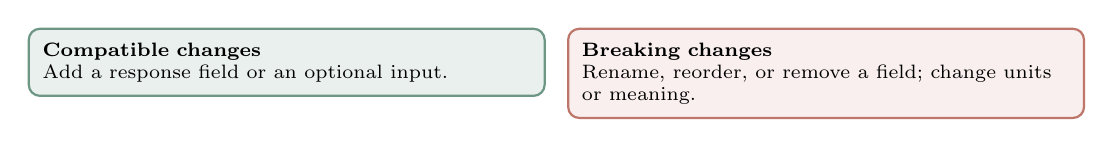
\begin{tikzpicture}
\node[tilegreen, anchor=north west, minimum width=6.55cm, text width=6.2cm, align=left, font=\scriptsize] at (0,0) {\textbf{Compatible changes}\\Add a response field or an optional input.};
\node[tilered, anchor=north west, minimum width=6.55cm, text width=6.2cm, align=left, font=\scriptsize] at (6.85,0) {\textbf{Breaking changes}\\Rename, reorder, or remove a field; change units or meaning.};
\end{tikzpicture}
\coursefooter
\end{cframe}

% ------------------------------------------------------------------ change scenarios
\newcommand{\scenmark}[3]{% column row code (0 none, 1 must change, 2 check)
  \ifcase#3\or\fill[courseblue] ({5.0+(#1-0.5)*1.15},{-#2*0.52}) circle (0.12);\or\draw[courseblue, line width=1.1pt] ({5.0+(#1-0.5)*1.15},{-#2*0.52}) circle (0.12);\fi
}
\newcommand{\scenrow}[9]{% row label c1 c2 c3 c4 c5 modular entangled
  \ifodd#1\else\fill[courseice!80] (0,{-#1*0.52-0.26}) rectangle (13.7,{-#1*0.52+0.26});\fi
  \node[anchor=west, text width=4.8cm, font=\scriptsize, align=left] at (0.05,{-#1*0.52}) {#2};
  \scenmark{1}{#1}{#3}\scenmark{2}{#1}{#4}\scenmark{3}{#1}{#5}\scenmark{4}{#1}{#6}\scenmark{5}{#1}{#7}
  \node[font=\small\bfseries, text=coursegreen] at (11.4,{-#1*0.52}) {#8};
  \node[font=\small\bfseries, text=coursered] at (12.85,{-#1*0.52}) {#9};
}
\begin{cframe}{Change scenarios: who has to change?}{\cterm{Feature}{an input variable.}\cterm{Threshold}{probability above which we decide ``fraud''.}\cterm{Gradient boosting}{many small trees added one by one.}\cterm{Entangled}{any change touches every part.}}
\centering
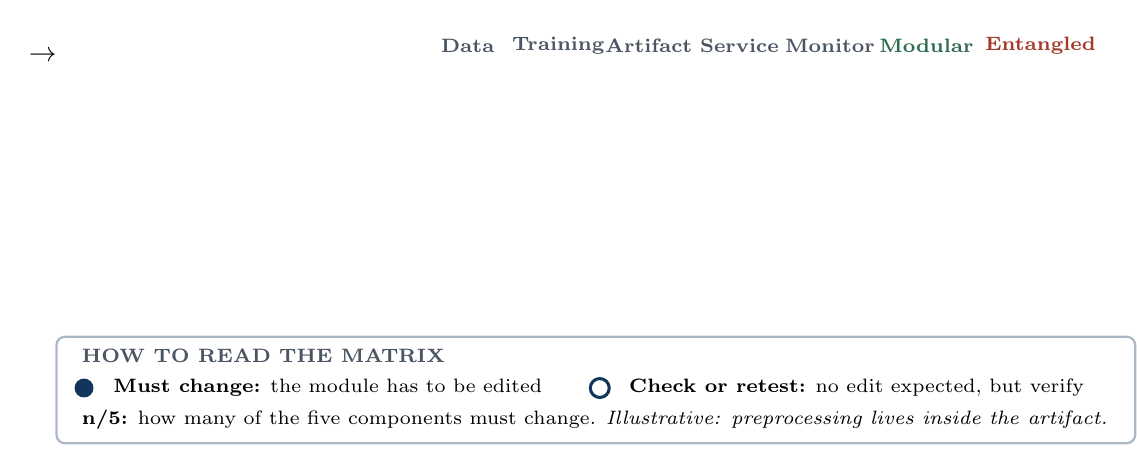
\begin{tikzpicture}
\foreach \i/\h in {1/Data,2/Training,3/Artifact,4/Service,5/Monitor} {
  \node[font=\scriptsize\bfseries, text=coursegray] at ({5.0+(\i-0.5)*1.15},0.2) {\h};
}
\node[font=\scriptsize\bfseries, text=coursegreen] at (11.4,0.2) {Modular};
\node[font=\scriptsize\bfseries, text=coursered] at (12.85,0.2) {Entangled};
\scenrow{1}{The data source is replaced}{1}{0}{0}{0}{2}{1/5}{5/5}
\scenrow{2}{A new derived feature is added}{1}{1}{1}{0}{2}{3/5}{5/5}
\scenrow{3}{Random forest $\to$ gradient boosting}{0}{1}{1}{2}{0}{2/5}{5/5}
\scenrow{4}{The response gets a new field}{0}{0}{0}{1}{2}{1/5}{5/5}
\scenrow{5}{The decision threshold changes}{0}{0}{0}{1}{2}{1/5}{5/5}
\scenrow{6}{The ML library is upgraded}{0}{1}{1}{1}{0}{3/5}{5/5}
% legend: same marks as the matrix
\draw[rounded corners=3pt, draw=courseblue!35, fill=white, thick] (0,-3.5) rectangle (13.7,-4.85);
\node[anchor=west, font=\scriptsize\bfseries, text=coursegray] at (0.2,-3.74) {HOW TO READ THE MATRIX};
\fill[courseblue] (0.35,-4.15) circle (0.12);
\node[anchor=west, font=\scriptsize] at (0.6,-4.15) {\textbf{Must change:} the module has to be edited};
\draw[courseblue, line width=1.1pt] (6.9,-4.15) circle (0.12);
\node[anchor=west, font=\scriptsize] at (7.15,-4.15) {\textbf{Check or retest:} no edit expected, but verify};
\node[anchor=west, font=\scriptsize] at (0.2,-4.55) {\textbf{n/5:} how many of the five components must change. \emph{Illustrative: preprocessing lives inside the artifact.}};
\end{tikzpicture}

\vspace{0.2em}
{\small Low coupling keeps each change inside one to three modules; the artifact is the boundary.}
\coursefooter
\end{cframe}

\begin{cframe}{Example: a prediction service as a pipeline of responsibilities}{\cterm{Endpoint}{one address of a service: method plus path, e.g.\ \texttt{POST /predict}.}\cterm{JSON}{a text format for structured data.}\cterm{Scaler}{rescales numeric features exactly as in training.}\cterm{Log}{a record of each request, kept for audit.}\cterm{curl}{a command-line tool that sends an HTTP request.}}
\centering
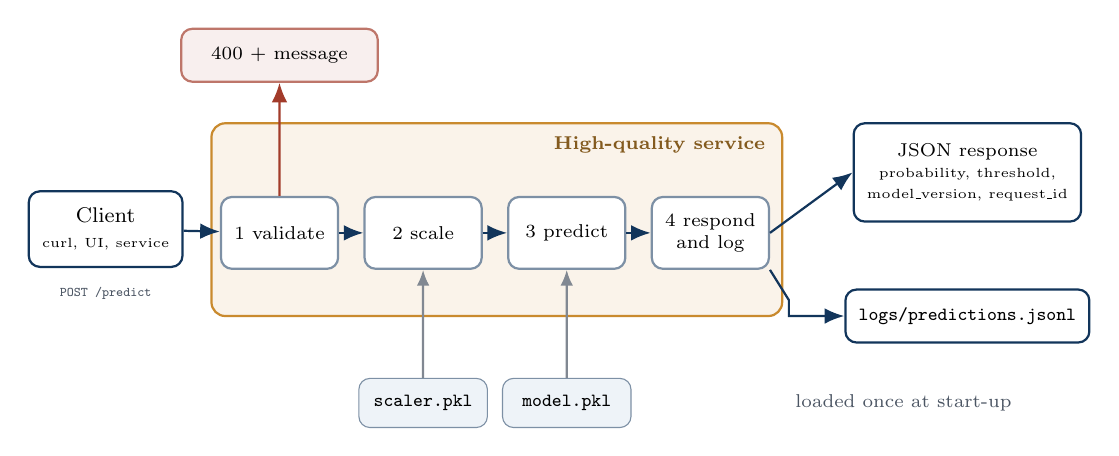
\begin{tikzpicture}[scale=0.96, transform shape]
\tikzset{st/.style={tileblue, minimum width=1.55cm, minimum height=0.95cm, font=\scriptsize, inner sep=2pt}}
\fill[coursegold!10, rounded corners=5pt, draw=coursegold, thick] (2.2,-1.0) rectangle (9.75,1.55);
\node[font=\scriptsize\bfseries, anchor=north east, text=coursegold!65!black] at (9.65,1.5) {High-quality service};
\node[tile, fill=white, draw=courseblue, thick, minimum width=1.6cm, minimum height=1.0cm] (cl) at (0.8,0.15) {Client\\{\tiny curl, UI, service}};
\node[st] (v) at (3.1,0.1) {1\ validate};
\node[st] (s) at (5.0,0.1) {2\ scale};
\node[st] (p) at (6.9,0.1) {3\ predict};
\node[st] (r) at (8.8,0.1) {4\ respond\\and log};
\node[tilered, minimum width=2.6cm, minimum height=0.7cm, font=\scriptsize] (err) at (3.1,2.45) {400 + message};
\node[tile, fill=white, draw=courseblue, thick, minimum width=2.7cm, minimum height=1.3cm, font=\scriptsize] (out) at (12.2,0.9) {JSON response\\{\tiny probability, threshold,}\\{\tiny model\_version, request\_id}};
\node[tile, fill=white, draw=courseblue, thick, minimum width=2.7cm, minimum height=0.7cm, font=\scriptsize] (log) at (12.2,-1.0) {\texttt{logs/predictions.jsonl}};
\node[tile, fill=courseice, draw=courseblue!55, minimum width=1.7cm, minimum height=0.65cm, font=\scriptsize] (sc) at (5.0,-2.15) {\texttt{scaler.pkl}};
\node[tile, fill=courseice, draw=courseblue!55, minimum width=1.7cm, minimum height=0.65cm, font=\scriptsize] (mo) at (6.9,-2.15) {\texttt{model.pkl}};
\draw[arrow] (cl) -- (v);
\node[font=\tiny\ttfamily, text=coursegray] at (0.8,-0.7) {POST /predict};
\draw[arrow] (v) -- (s); \draw[arrow] (s) -- (p); \draw[arrow] (p) -- (r);
\draw[arrowred] (v) -- (err);
\draw[arrow] (r.east) -- (out.west);
\draw[arrow] (r.south east) -- ++(0.25,-0.4) |- (log.west);
\draw[arrowgray] (sc) -- (s);
\draw[arrowgray] (mo) -- (p);
\node[note, anchor=west] at (9.8,-2.15) {loaded once at start-up};
\end{tikzpicture}
\coursefooter
\end{cframe}

% ------------------------------------------------------------------ testing
\sectiondivider{5}{Quality assurance}{separating what changes and agreeing on contracts keeps change cheap.}{$\bullet$\ Testing levels\\[3pt]$\bullet$\ Testing ML systems: code, data, and models\\[3pt]$\bullet$\ Evidence: the same six requests sent to two implementations}

\begin{cframe}{Testing levels}{\cterm{Unit test}{checks one small piece.}\cterm{Integration test}{checks parts working together.}\cterm{Acceptance test}{checks a requirement.}\cterm{Regression}{a change breaks what used to work.}}
\centering
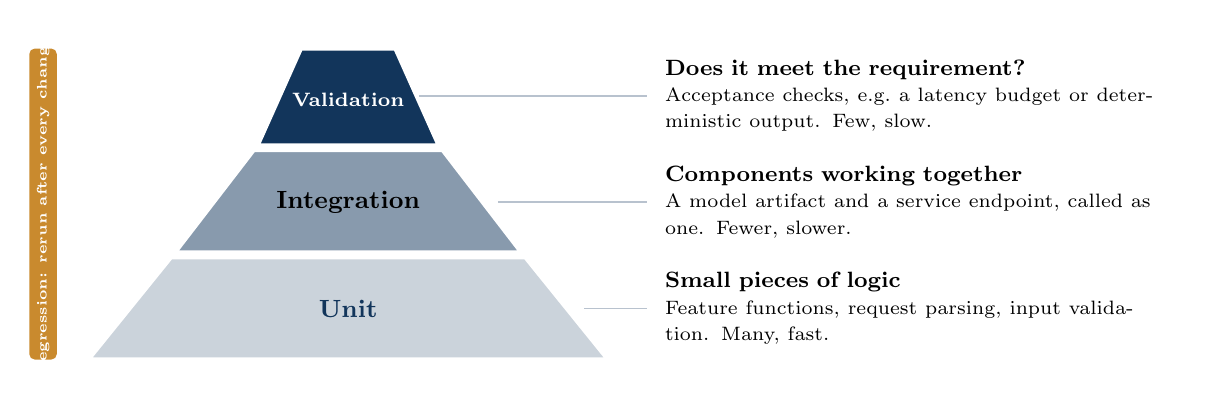
\begin{tikzpicture}
% pyramid
\fill[courseblue!22, draw=white, line width=1.5pt] (0,0) -- (6.6,0) -- (5.55,1.3) -- (1.05,1.3) -- cycle;
\fill[courseblue!50, draw=white, line width=1.5pt] (1.1,1.36) -- (5.5,1.36) -- (4.5,2.66) -- (2.1,2.66) -- cycle;
\fill[courseblue, draw=white, line width=1.5pt] (2.15,2.72) -- (4.45,2.72) -- (3.9,3.95) -- (2.7,3.95) -- cycle;
\node[font=\small\bfseries, text=courseblue] at (3.3,0.65) {Unit};
\node[font=\small\bfseries, text=black] at (3.3,2.0) {Integration};
\node[font=\scriptsize\bfseries, text=white] at (3.3,3.3) {Validation};
% regression bar
\fill[coursegold, rounded corners=2pt] (-0.75,0) rectangle (-0.4,3.95);
\node[font=\tiny\bfseries, text=white, rotate=90] at (-0.575,1.98) {regression: rerun after every change};
% labels
\node[anchor=west, text width=6.4cm, font=\footnotesize, align=left] at (7.2,0.65) {\textbf{Small pieces of logic}\\{\scriptsize Feature functions, request parsing, input validation. Many, fast.}};
\node[anchor=west, text width=6.4cm, font=\footnotesize, align=left] at (7.2,2.0) {\textbf{Components working together}\\{\scriptsize A model artifact and a service endpoint, called as one. Fewer, slower.}};
\node[anchor=west, text width=6.4cm, font=\footnotesize, align=left] at (7.2,3.35) {\textbf{Does it meet the requirement?}\\{\scriptsize Acceptance checks, e.g.\ a latency budget or deterministic output. Few, slow.}};
\draw[courseblue!30, line width=0.6pt] (6.3,0.65) -- (7.1,0.65);
\draw[courseblue!30, line width=0.6pt] (5.2,2.0) -- (7.1,2.0);
\draw[courseblue!30, line width=0.6pt] (4.2,3.35) -- (7.1,3.35);
\end{tikzpicture}
\coursefooter
\end{cframe}

\newcommand{\testcard}[7]{% index x headcolor title line1 line2 line3
  \node[rounded corners=4pt, fill=#3, text=white, minimum width=4.3cm, minimum height=0.75cm, font=\small\bfseries, anchor=north west] (h#1) at (#2,0) {#4};
  \node[tile, fill=courseice, anchor=north west, minimum width=4.3cm, minimum height=2.75cm, text width=3.95cm, align=left, font=\footnotesize] at ([yshift=-0.06cm]h#1.south west) {$\bullet$\ #5\\[5pt]$\bullet$\ #6\\[5pt]$\bullet$\ #7};
}
\begin{cframe}{Testing ML systems: code, data, and models}{\cterm{Held-out data}{examples kept out of training and used only to evaluate.}\cterm{Slice}{a subset of the data, e.g.\ one region.}\cterm{Invariance test}{a small irrelevant change must not change the prediction.}}
\centering

\begin{tikzpicture}
\testcard{1}{0}{courseblue}{Code}{Unit and integration tests, as in any software.}{Does the service reject invalid input?}{Does the pipeline run end to end?}
\testcard{2}{4.55}{coursegold!80!black}{Data}{Schema, ranges, and missing values are checked.}{Training and serving data are compared.}{A bad batch stops the pipeline early.}
\testcard{3}{9.1}{coursegreen}{Model}{Metrics on held-out data, overall and per slice.}{Behavior under small input changes.}{Comparison with the previous model.}
\node[font=\scriptsize, text=coursegray, anchor=north west] at (0,-3.95) {After Breck et al., The ML Test Score (2017).};
\end{tikzpicture}
\coursefooter
\end{cframe}

\begin{cframe}{Evidence: the same six requests sent to two implementations}{\cterm{NaN}{``not a number'': a missing or undefined numeric value.}\cterm{Silent failure}{a wrong answer that looks fine.}\cterm{Crash}{the service fails visibly, with HTTP 500.}\cterm{Test client}{calls the service inside a test, without a network.}}
\centering
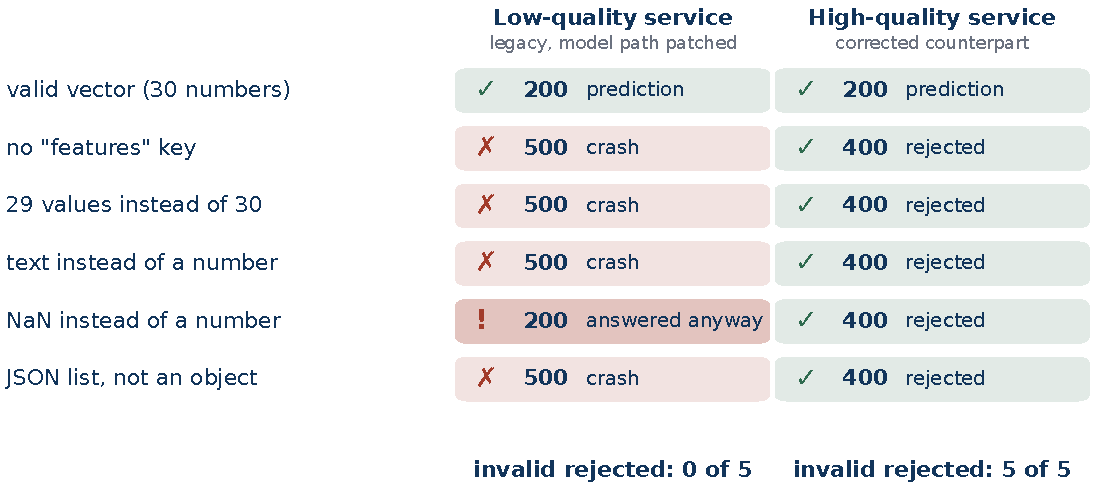
\includegraphics[width=0.9\textwidth,height=0.6\textheight,keepaspectratio]{images/class20_api_behavior.pdf}

{\scriptsize\color{coursegray} Flask test client; the low-quality service ran with \texttt{streamlit/model.pkl} standing in for its missing pickle.}

\vspace{0.3em}

\begin{tikzpicture}
\node[tilegold, minimum width=13.4cm, text width=13.0cm, font=\small] {\textbf{A crash is visible; a wrong answer is not:} the low-quality service answers 200 for NaN.};
\end{tikzpicture}
\coursefooter
\end{cframe}

% ------------------------------------------------------------------ maintenance
\sectiondivider{6}{Evolution and MLOps}{tests tell us whether the system still works as it changes.}{$\bullet$\ Maintenance and evolution: four kinds of change\\[3pt]$\bullet$\ Software costs more to keep than to build\\[3pt]$\bullet$\ Reproducibility needs configuration management\\[3pt]$\bullet$\ From DevOps to MLOps: two loops\\[3pt]$\bullet$\ From notebook to production: a ladder of discipline}

\begin{cframe}{Maintenance and evolution: four kinds of change}{\cterm{Retraining}{fitting the model again on newer data.}\cterm{Schema change}{a change in the structure of the data.}\cterm{Refactoring}{restructuring code without changing what it does.}}
\centering
\begin{tikzpicture}
\ptile{0}{0}{tileblue}{Corrective}{Fix defects found in use.}{a feature function that mishandles missing values.}
\ptile{6.85}{0}{tileblue}{Adaptive}{Keep working as the environment changes.}{retraining on new data, a library upgrade, a schema change.}
\ptile{0}{-2.6}{tileblue}{Perfective}{Add or improve capabilities.}{a new feature, a better model, a lower latency.}
\ptile{6.85}{-2.6}{tilegold}{Preventive}{Reduce the cost of future change.}{refactoring, tests, documentation, pipeline cleanup.}
\end{tikzpicture}
\coursefooter
\end{cframe}

% ------------------------------------------------------------------ cost
\begin{cframe}{Software costs more to keep than to build}{\cterm{Maintenance}{all work on a system after its first release.}\cterm{Cumulative cost}{total cost accumulated over time.}}
\begin{columns}[T]
\column{0.55\textwidth}
\centering
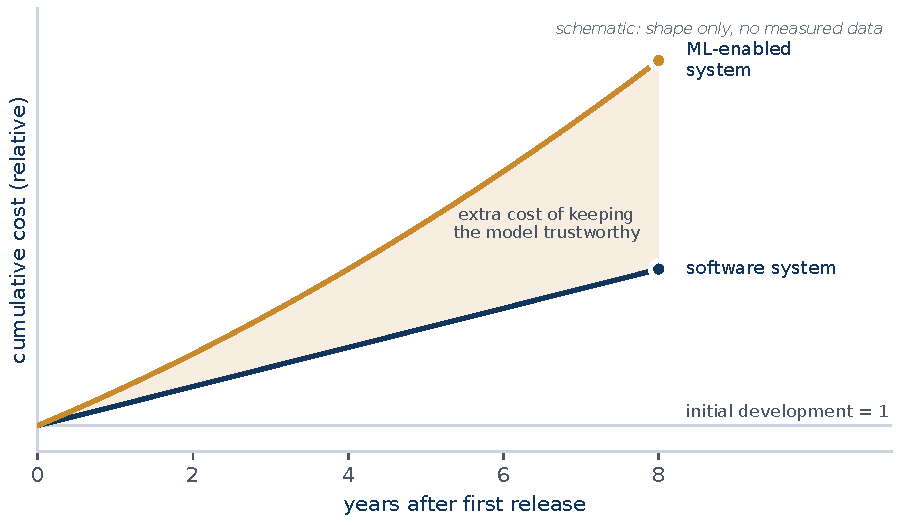
\includegraphics[width=\textwidth]{images/class20_cost_schematic.pdf}

{\scriptsize\color{coursegray}\raggedright Sources: Sommerville, \emph{Software Engineering}; Glass (2002), Fact 41: maintenance is 40--80\% of software cost; Sculley et al.\ (2015), for ML systems.\par}
\column{0.43\textwidth}
\begin{itemize}\small
\item Software often costs more to maintain than to develop.
\item Requirements change as users learn what they really need.
\item In ML systems, data work, monitoring, and retraining push the maintenance share even higher.
\end{itemize}
\end{columns}
\coursefooter
\end{cframe}

% ------------------------------------------------------------------ configuration management
\newcommand{\cfgtile}[4]{% index y title detail
  \node[tileblue, anchor=west, minimum width=4.6cm, minimum height=0.95cm, text width=4.2cm, align=left] (c#1) at (0,#2) {\textbf{\color{courseblue}#3}\\{\scriptsize\color{coursegray}#4}};
}
\begin{cframe}{Reproducibility needs configuration management}{\cterm{Configuration management}{versioning everything that defines a result.}\cterm{Seed}{a number that makes randomness repeatable.}\cterm{Experiment tracking}{a record of each training run.}\cterm{Hash}{a short fingerprint of a file, used as a version.}}
\centering
\begin{tikzpicture}
\cfgtile{1}{3.4}{Code}{a Git commit (Class 17)}
\cfgtile{2}{2.28}{Data}{a dataset version or hash}
\cfgtile{3}{1.16}{Configuration}{hyperparameters and seeds}
\cfgtile{4}{0.04}{Environment}{library and runtime versions}
\node[tilegold, minimum width=3.0cm, minimum height=1.4cm, font=\small] (model) at (8.0,1.72) {\textbf{Trained model}\\{\scriptsize a versioned artifact (Class 19)}};
\node[tileblue, minimum width=2.6cm, minimum height=1.4cm, font=\small] (pred) at (12.1,1.72) {\textbf{Prediction}\\{\scriptsize carries the model version}};
\foreach \i in {1,2,3,4} {\draw[arrowgold] (c\i.east) -- (model.west);}
\draw[arrow] (model.east) -- (pred.west);
\end{tikzpicture}

\vspace{0.3em}
\begin{itemize}\small
\item \textbf{Reproducible:} the same four inputs give the same model.
\item \textbf{Traceable:} any prediction can be followed back to all four. Experiment tracking (Class 19) records them together.
\end{itemize}
\coursefooter
\end{cframe}

% ------------------------------------------------------------------ DevOps -> MLOps
\newcommand{\loopbox}[4]{% x y style label
  \node[#3, minimum width=2.3cm, minimum height=0.85cm, font=\small\bfseries] (#4) at (#1,#2) {#4};
}
\begin{cframe}{From DevOps to MLOps: two loops}{\cterm{DevOps}{development and operations working as one loop to build, test, release, and run software.}\cterm{MLOps}{DevOps plus the model lifecycle: data, training, evaluation, registry, monitoring.}\cterm{CI/CD}{automatic build, test, and release.}\cterm{Drift}{data changes and the model degrades.}}
\centering
\begin{tikzpicture}[scale=0.88, transform shape]
\node[font=\scriptsize\bfseries, text=courseblue, anchor=west] at (0,3.35) {SOFTWARE LOOP (DEVOPS): REPEATED ON EVERY CHANGE};
\loopbox{1.15}{2.6}{tileblue}{Code}
\loopbox{3.85}{2.6}{tileblue}{Build}
\loopbox{6.55}{2.6}{tileblue}{Test}
\loopbox{9.25}{2.6}{tileblue}{Release}
\loopbox{11.95}{2.6}{tileblue}{Operate}
\loopbox{1.15}{0.3}{tilegold}{Data}
\loopbox{3.85}{0.3}{tilegold}{Train}
\loopbox{6.55}{0.3}{tilegold}{Evaluate}
\loopbox{9.25}{0.3}{tilegold}{Register}
\loopbox{11.95}{0.3}{tilegold}{Monitor}
\foreach \a/\b in {Code/Build,Build/Test,Test/Release,Release/Operate} {\draw[arrow] (\a) -- (\b);}
\foreach \a/\b in {Data/Train,Train/Evaluate,Evaluate/Register,Register/Monitor} {\draw[arrowgold] (\a) -- (\b);}
\foreach \a/\b in {Code/Data,Build/Train,Test/Evaluate,Release/Register,Operate/Monitor} {\draw[coursegray!70, thick, <->] (\a.south) -- (\b.north);}
\node[font=\scriptsize\bfseries, text=coursegold!65!black, anchor=west] at (0,-0.5) {MODEL LOOP (ADDED BY ML): REPEATED ON EVERY NEW DATA OR RETRAINING};
\node[tag, anchor=north east] at (13.6,3.75) {PREVIEW OF CLASS 26};
\node[tileblue, anchor=north west, minimum width=13.4cm, text width=13.0cm, align=left, font=\small] at (0,-0.95) {\textbf{CI/CD} builds, tests, and releases every change automatically; for ML, the data and the model artifact are checked as well.};
\node[tilegreen, anchor=north west, minimum width=13.4cm, text width=13.0cm, align=left, font=\small] at (0,-2.05) {\textbf{MLOps} runs both loops together, automated and observable.};
\end{tikzpicture}
\coursefooter
\end{cframe}

% ------------------------------------------------------------------ maturity ladder
\newcommand{\ladder}[7]{% index height fill textcolor title path gain
  \pgfmathsetmacro{\xx}{(#1-1)*2.7}
  \fill[rounded corners=3pt, fill=#3] (\xx,0) rectangle (\xx+2.6,#2);
  \node[anchor=north west, text width=2.35cm, font=\footnotesize, text=#4, align=left] at (\xx+0.1,#2-0.1) {\textbf{#5}\\[1pt]{\scriptsize #6}};
  \node[anchor=north west, text width=2.5cm, font=\scriptsize, text=coursegray, align=left] at (\xx+0.02,-0.1) {#7};
}
\begin{cframe}{From notebook to production: a ladder of discipline}{\cterm{Docker}{packages a program with its environment so it runs the same anywhere.}\cterm{GitHub Actions, Jenkins}{tools that run automated pipelines on every change.}}
\centering
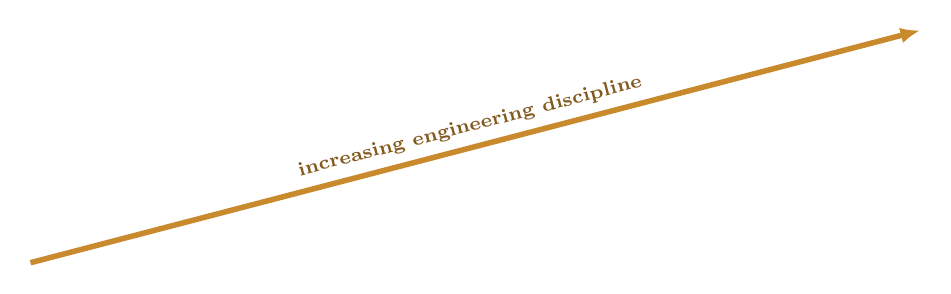
\begin{tikzpicture}
\ladder{1}{1.4}{courseblue!10}{black}{Notebook}{Jupyter, pandas,\\scikit-learn}{explore and explain}
\ladder{2}{2.0}{courseblue!22}{black}{Training script}{Python scripts,\\scikit-learn}{repeat the training}
\ladder{3}{2.6}{courseblue!40}{black}{Saved artifact}{pickle, Git,\\Weights \& Biases}{reuse and version}
\ladder{4}{3.2}{courseblue!65}{white}{Service}{Flask,\\HTTP and JSON}{a contract others can call}
\ladder{5}{3.8}{courseblue}{white}{Automated delivery}{Docker, GitHub\\Actions, Jenkins}{ship it repeatably}
\draw[arrowgold, line width=2pt] (0.1,2.0) -- (11.4,4.95) node[midway, sloped, above, font=\scriptsize\bfseries, text=coursegold!65!black] {increasing engineering discipline};
\end{tikzpicture}
\coursefooter
\end{cframe}

\section{Wrap-up}\gdef\currentsectionname{Wrap-up}

% ------------------------------------------------------------------ reading
\begin{frame}{Papers and materials}
\readinglist{
\href{https://www.pearson.com/en-us/subject-catalog/p/software-engineering/P200000003144/9780137035151}{Sommerville, Software Engineering};\
\href{https://www.informit.com/store/facts-and-fallacies-of-software-engineering-9780321117427}{Glass, Facts and Fallacies of Software Engineering (2002)};\\
\href{https://abseil.io/resources/swe-book}{Winters, Manshreck, and Wright, Software Engineering at Google};\
\href{https://doi.org/10.1145/361598.361623}{Parnas, On the Criteria to Be Used in Decomposing Systems into Modules (1972)};\
\href{https://proceedings.neurips.cc/paper/2015/file/86df7dcfd896fcaf2674f757a2463eba-Paper.pdf}{Sculley et al., Hidden Technical Debt in Machine Learning Systems};\
\href{https://research.google/pubs/the-ml-test-score-a-rubric-for-ml-production-readiness-and-technical-debt-reduction/}{Breck et al., The ML Test Score};\
\href{https://arxiv.org/abs/2110.10234}{Nahar et al., Collaboration Challenges in Building ML-Enabled Systems};\
\href{https://www.oreilly.com/library/view/designing-machine-learning/9781098107956/}{Chip Huyen, Designing Machine Learning Systems};\
\href{https://martinfowler.com/articles/microservice-trade-offs.html}{Martin Fowler, trade-offs in architecture}.
}
\coursefooter
\end{frame}

\classclosingframe
{\begin{itemize}
\item Model quality and software quality are related but not interchangeable.
\item Boundaries, tests, and versioned artifacts make an ML idea a dependable system.
\item MLOps automates today's loops; it does not replace the engineering behind them.
\end{itemize}}
{Review your project with the same lenses: requirements, boundaries, tests, versioning, monitoring.}
{Class 21 is a guest session (Cybertec). Class 22 turns needs and quality attributes into testable requirements.}
{Engineering discipline around code and process sets up the same discipline around requirements: knowing what ``good'' means before we build.}

\appendix

% ------------------------------------------------------------------ backup
\begin{cframe}{Backup: design smells in ML projects}{\cterm{Smell}{a sign in the code that hints at a deeper design problem.}\cterm{Boundary}{the point where data enters a module.}}
\centering
\renewcommand{\arraystretch}{1.2}
\setlength{\tabcolsep}{5pt}
{\footnotesize
\begin{tabularx}{\textwidth}{>{\raggedright\arraybackslash}p{4.9cm} >{\raggedright\arraybackslash}p{3.3cm} >{\raggedright\arraybackslash}X}
\rowcolor{courseblue}
\color{white}\textbf{Smell} & \color{white}\textbf{Principle at stake} & \color{white}\textbf{Refactoring} \\
A bare list of numbers whose order only the author knows & Implicit contract & Named fields, validated at the boundary \\
\rowcolor{courseice}
The decision threshold is implicit: whatever \texttt{predict()} does & Configuration mixed with logic & An explicit, documented setting \\
One function loads data, cleans it, trains, plots, and saves & Low cohesion & One responsibility per step, composed in a pipeline \\
\rowcolor{courseice}
The service imports code from the training notebook & Coupling to internals & Share only the artifact and its schema \\
Notebook cells depend on variables defined many cells earlier & Hidden dependency & Functions with explicit inputs and outputs \\
\rowcolor{courseice}
Retraining is a manual sequence of notebook cells & No automation boundary & A script with explicit inputs and outputs that a scheduler can run \\
\end{tabularx}}

\vspace{0.5em}
{\scriptsize In the high-quality service: an explicit threshold (\texttt{FRAUD\_THRESHOLD}) and input validated at the boundary.}
\coursefooter
\end{cframe}

\end{document}
